\chapter{Quicksort}
\label{ch:quicksort}

\newcommand{\lecnum}{7}
%\newcommand{\lectitle}{Quicksort}
\newcommand{\lecturer}{Frank Pfenning}

\chapterTAGS{average-cost, complexity, correctness, divide-and-conquer, safety, sorting}
\maketitle

\begin{preamble}
In this lecture we consider two related algorithms for sorting that achieve a
much better running time than the selection sort from an earlier lecture:
mergesort and quicksort.  We develop quicksort and its invariants in detail.
As usual, contracts and loop invariants will bridge the gap between the
abstract idea of the algorithm and its implementation.
\end{preamble}

\begin{gram}[Learning Goals]
We will revisit many of the computational thinking, algorithm, and
programming concepts from the previous lectures.  We highlight
the following important ones:
\begin{description}
\item[Computational Thinking: ]%
  We revisit the divide-and-conquer technique from the lecture on binary
  search.  We will also see the importance of \emph{randomness} for the first
  time.
\item[Algorithms and Data Structures: ]%
  We examine mergesort and quicksort, both of which use divide-and-conquer,
  but with different overall strategies.
\item[Programming: ]%
  We have occasionally seen \emph{recursion} in specification functions.  In
  both mergesort and quicksort, it will be a central computational technique.
\end{description}
\end{gram}

Both mergesort and quicksort are examples of \emph{divide-and-conquer}.  We
divide a problem into simpler subproblems that can be solved independently and
then combine the solutions.  As we have seen for binary search, the ideal
\emph{divide} step breaks a problem into two of roughly equal size, because it
means we need to divide only logarithmically many times before we have a basic
problem, presumably with an immediate answer.  Mergesort achieves this,
quicksort not quite, which presents an interesting trade-off when considering
which algorithm to chose for a particular class of applications.

Recall linear search for an element in an array, which has asymptotic
complexity of $O(n)$.  The divide-and-conquer technique of binary
search divides the array in half, determines which half our element
would have to be in, and then proceeds with only that subarray.  An
interesting twist here is that we \emph{divide}, but then we need to
\emph{conquer} only a single new subproblem.  So if the length of the
array is $2^k$ and we divide it by two on each step, we need at most
$k$ iterations.  Since there is only a constant number of operations
on each iteration, the overall complexity is $O(\log n)$.  As a side
remark, if we divided the array into 3 equal sections, the complexity
would remain $O(\log n)$ because $3^k = (2^{\log_2 3})^k = 2^{\log_2 3
  \times k}$, so $\log_2 n$ and $\log_3 n$ only differ in a constant
factor, namely $\log_2 3$.


\section{The Quicksort Algorithm}
\label{sec:quicksort:concept}
\TAGS{average-cost, complexity, divide-and-conquer, sorting}

Quicksort uses the technique of divide-and-conquer in a different
manner.  We proceed as follows:
\begin{enumerate}
\item Pick an arbitrary element of the array (the \emph{pivot}).
\item Divide the array into two segments, the elements that are smaller than
  the pivot and the elements that are greater, with the pivot in between (the
  \emph{partition} phase).
\item Recursively sort the segments to the left and right
  of the pivot.
\end{enumerate}
In quicksort, dividing the problem into subproblems will be linear
time, but putting the results back together is immediate.  This kind
of trade-off is frequent in algorithm design.

Let us analyze the asymptotic complexity of the partitioning
phase of the algorithm.  Say we have the array
$$
3,1,4,4,7,2,8
$$
and we pick $3$ as our pivot.  Then we have to compare each element of this
(unsorted!) array to the pivot to obtain a partition where $2, 1$ are to the
left and $4, 7, 8, 4$ are to the right of the pivot.  We have picked an
arbitrary order for the elements in the array segments: all that matters is
that all smaller ones are to the left of the pivot and all larger ones are to
the right.

Since we have to compare each element to the pivot, but otherwise just collect
the elements, it seems that the partition phase of the algorithm should have
complexity $O(k)$, where $k$ is the length of the array segment we have to
partition.

It should be clear that in the ideal (best) case, the pivot element will be
magically the \emph{median} value among the array values.  This just means
that half the values will end up in the left partition and half the values
will end up in the right partition.  So we go from the problem of sorting an
array of length $n$ to an array of length $n/2$.  Repeating this process, we
obtain the following picture:
\begin{center}
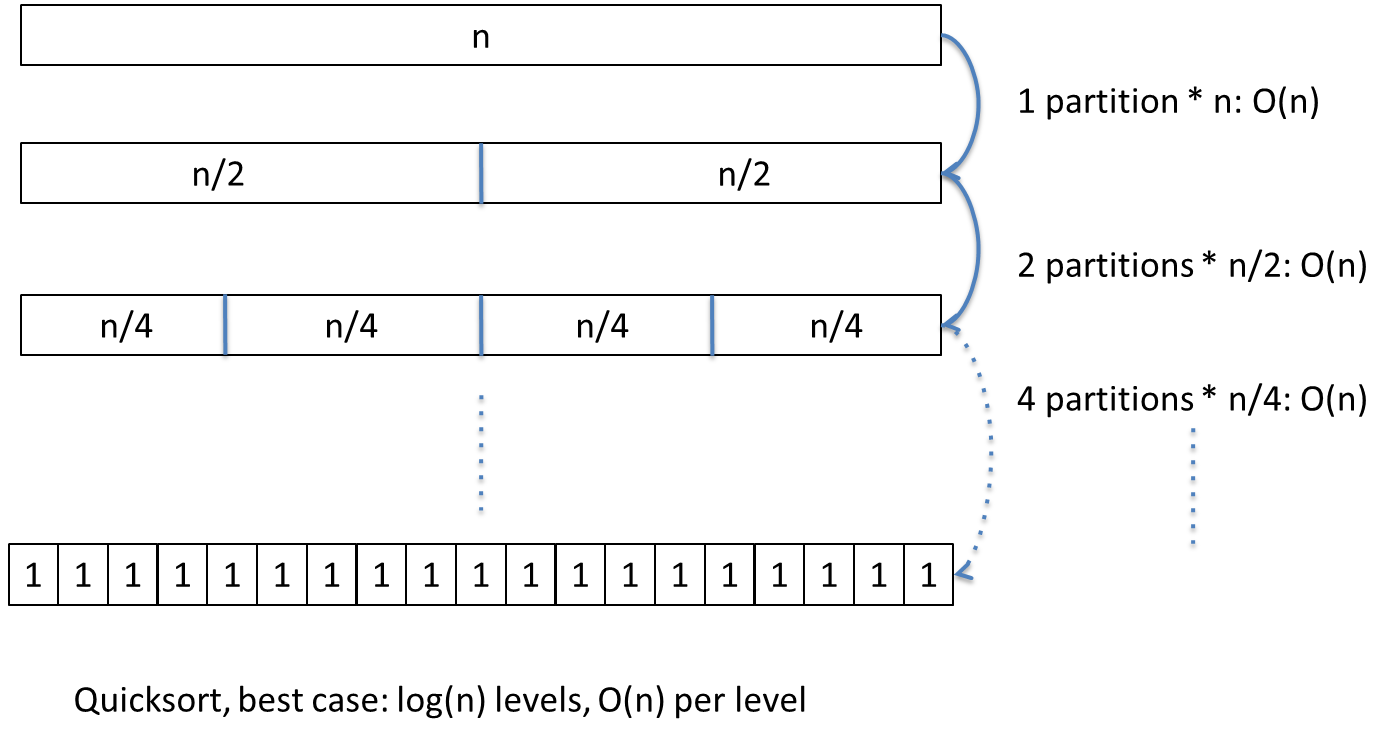
\includegraphics[width=0.99\textwidth]{img/qsort1.png}
\end{center}
At each level the total work is $O(n)$ operations to perform the partition.
In the best case there will be $O(\log n)$ levels, leading us to the
$O(n \log n)$ best-case asymptotic complexity.

How many recursive calls do we have in the worst case, and how long are the
array segments?  In the worst case, we always pick either the smallest or
largest element in the array so that one side of the partition will be empty,
and the other has all elements except for the pivot itself.  In the example
above, the recursive calls might proceed as follows (where we have surrounded
the unsorted part of the array with brackets):
$$
\begin{array}{ll}
      \text{array} & \text{pivot}
\\\hline
   [3,1,4,4,8,2,7] & 1
\\ 1,[3,4,4,8,2,7] & 2
\\ 1,2,[3,4,4,8,7] & 3
\\ 1,2,3,[4,4,8,8] & 4
\\ 1,2,3,4,[4,8,7] & 4
\\ 1,2,3,4,4,[8,7] & 7
\\ 1,2,3,4,4,7,[8]
\end{array}
$$
All other recursive calls are with the empty array segment, since we
never have any unsorted elements less than the pivot.  We see that in
the worst case there are $n-1$ significant recursive calls for an
array of size $n$.  The $k$-th recursive call has to sort a subarray of
size $n-k$, which proceeds by partitioning, requiring $O(n-k)$
comparisons.

This means that, overall, for some constant $c$ we have
$$
c\sum_{k = 0}^{n-1} k = c\frac{n(n-1)}{2} \in O(n^2)
$$
comparisons.  Here we used the fact that $O(p(n))$ for a polynomial $p(n)$ is
always equal to the $O(n^k)$ where $k$ is the leading exponent of the
polynomial.  This is because the largest exponent of a polynomial will
eventually dominate the function, and big-O notation ignores constant
coefficients.

So quicksort has quadratic complexity in the worst case.  How can we
mitigate this?  If we could always pick the \emph{median} among the
elements in the subarray we are trying to sort, then half the elements
would be less and half the elements would be greater.  So in this case
there would be only $\log n$ recursive calls, where at each layer we
have to do a total amount of $n$ comparisons, yielding an asymptotic
complexity of $O(n \log n)$.

Unfortunately, it is not so easy to compute the median to obtain the
optimal partitioning. It \emph{is} possible to compute the median of
$n$ elements in $O(n)$ time, but quicksort is rarely if ever
implemented this way in practice. One reason for this is that it turns
out that if we pick a \emph{random} element, the algorithm will run in
$O(n\log n)$ time most of the time.

Randomness is very important if we want to claim the algorithm is likely to
run in $O(n\log n)$ time. With any fixed-pick strategy, there will be
sample inputs on which the algorithm takes $O(n^2)$ steps.  For example, if we
always pick the first element, then if we supply an array that is already
sorted, quicksort will take $O(n^2)$ steps (and similarly if it is ``almost''
sorted with a few exceptions)!  If we pick the pivot randomly each time, the
kind of array we get does not matter: the expected running time is always the
same, namely $O(n\log n)$. It's still \emph{possible} that we could
randomly pick bad pivots, but probabilistically, the chance of this is very,
very low.  Proving this, however, is a different matter and beyond the scope
of this course.  This is an important example on how to exploit randomness to
obtain a reliable average case behavior, no matter what the distribution of
the input values.


\section{The Quicksort Function}
\label{sec:quicksort:function}
\TAGS{correctness, divide-and-conquer, safety, sorting}

We now turn our attention to developing an imperative implementation
of quicksort, following our high-level description.  We implement
quicksort in the function \lstinline'sort' as an \emph{in-place}
sorting function that modifies a given array instead of creating
a new one.  It therefore returns no value, which is expressed
by giving a return type of \lstinline'void'.
\begin{lstlisting}[language={[C0]C}, numbers=left]
void sort(int[] A, int lo, int hi)
//@requires 0 <= lo && lo <= hi && hi <= \length(A);
//@ensures is_sorted(A, lo, hi);
{
  ...
}
\end{lstlisting}
Quicksort solves the same problem as selection sort, so their contract is the same, but their implementation differs.
We sort the segment $A\lbrack\mathit{lo}..\mathit{hi})$ of the array
between $\mathit{lo}$ (inclusively) and $\mathit{hi}$
(exclusively).  The precondition in the \requires{} annotation
verifies that the bounds are meaningful with respect to $A$.
The post-condition in the \ensures{} clause guarantees
that the given segment is sorted when the function returns.
It does not express that the output is a permutation of the
input, which is required to hold but is not formally expressed
in the contract (see Exercise~\ref{exc:is-permutation}).


The quicksort function represents an example of \emph{recursion}: a
function (\lstinline'sort') calls itself on a smaller argument.  When
we analyze such a function call, it would be a mistake to try to
analyze the function that we call recursively.  Instead, we reason
about it using \emph{contracts}.
\begin{enumerate}
\item We have to ascertain that the preconditions of the function
  we are calling are satisfied.
\item We are allowed to assume that the post-conditions of the
  function we are calling are satisfied when it returns.
\end{enumerate}
This applies no matter whether the call is recursive, as it is in
this example, or not.

Reasoning about recursive functions using their contracts is an
excellent illustration of computational thinking, separating the
\emph{what} (that is, the contract) from the \emph{how} (that is, the
definition of the function).  To analyze the recursive call we only
care about \emph{what} the function does.

We also need to analyze the \emph{termination} behavior of the
function, verifying that the recursive calls are on strictly smaller
arguments.  What \emph{smaller} means differs for different functions;
here the size of the subrange of the array is what decreases.  The
quantity $\mathit{hi}-\mathit{lo}$ is divided by two for each
recursive call and is therefore smaller since it is always greater or
equal to $2$.  If it were less than $2$ we would return immediately
and not make a recursive call.


For quicksort, we don't have to do anything if we
have an array segment with 0 or 1 elements.  So we just return
if $\mathit{hi}-\mathit{lo} \leq 1$.

\begin{lstlisting}[language={[C0]C}, numbers=left]
void sort(int[] A, int lo, int hi)
//@requires 0 <= lo && lo <= hi && hi <= \length(A);
//@ensures is_sorted(A, lo, hi);
{
  if (hi-lo <= 1) return;
  ...
}
\end{lstlisting}

\clearpage
Next we have to select a pivot element and call a partition function.
We tell that function the index of the element that we chose as the pivot.
For illustration purposes, we use the middle element as a pivot (to
work reasonably well for arrays that are sorted already), but it
should really be a random element.
We want partitioning to be done \emph{in place}, modifying the array
$A$.  Still, partitioning needs to return the index $\mathit{mid}$ of the pivot
element because we then have to recursively sort the two subsegments
to the left and right of the index where the pivot is after partitioning.
So we declare:
\begin{lstlisting}[language={[C0]C}, numbers=left]
int partition(int[] A, int lo, int pi, int hi)
//@requires 0 <= lo && lo <= pi;
//@requires pi < hi && hi <= \length(A);
//@ensures lo <= \result && \result < hi;
//@ensures ge_seg(A[\result], A, lo, \result);
//@ensures le_seg(A[\result], A, \result+1, hi);
  ;
\end{lstlisting}
Here we use the auxiliary functions \lstinline'ge_seg' (for \emph{greater
  or equal than segment}) and \lstinline'le_seg' (for \emph{less or equal
  than segment}), where
\begin{itemize}
\item \lstinline'ge_seg(x, A, lo, mid)' if $x \geq y$ for every $y$ in
  $A\lbrack\mathit{lo}{..}\mathit{mid})$.
\item \lstinline'le_seg(x, A, mid+1, hi)' if $x \leq y$ for every $y$
  in $A\lbrack\mathit{mid}{+}1{..}\mathit{hi})$.
\end{itemize}
Their definitions can be found in file \lstinline'arrayutil.c0'.

Some details on this specification: we require $\mathit{pi}$ to be a valid index in the array range, i.e., $\mathit{lo} \leq \mathit{pi} <
\mathit{hi}$. In particular, we require $\mathit{lo} <
\mathit{hi}$ because if they were equal, then the segment could be
empty and we cannot possibly pick a pivot element or return its index.
%We ensure that $\mathit{result} < hi$ so that the index of the
%pivot is a legal index in the segment
%$A[\mathit{lo}..\mathit{hi})$.

Now we can fill in the remainder of the main sorting function.
\clearpage
\begin{lstlisting}[language={[C0]C}, numbers=left]
void sort(int[] A, int lo, int hi)
//@requires 0 <= lo && lo <= hi && hi <= \length(A);
//@ensures is_sorted(A, lo, hi);
{
  if (hi-lo <= 1) return;
  int pi = lo + (hi-lo)/2; /* should be random */

  int mid = partition(A, lo, pi, hi);
  sort(A, lo, mid);
  sort(A, mid+1, hi);
  return;
}
\end{lstlisting}
It is a simple but instructive exercise to reason about this program,
using only the contract for \lstinline'partition' together with the pre-
and post-conditions for \lstinline'sort' (see
Exercise~\ref{exc:qsort-post}).

To show that the \lstinline'sort' function terminates, we have to show the
array segment becomes strictly smaller in each recursive call.  First,
$\mathit{mid}-\mathit{lo} < \mathit{hi}-\mathit{lo}$ since
$\mathit{mid} < \mathit{hi}$ by the post-condition for
\lstinline'partition'.  Second, $\mathit{hi}-(\mathit{mid}+1) <
\mathit{hi}-\mathit{lo}$ because $\mathit{lo} <
\mathit{mid}+1$, also by the post-condition for \lstinline'partition'.


\section{Partitioning}
\label{sec:quicksort:partitioning}
\TAGS{safety}

The trickiest aspect of quicksort is the partitioning step, in
particular since we want to perform this operation in place.
Let's consider the situation when partition is called:
\begin{center}
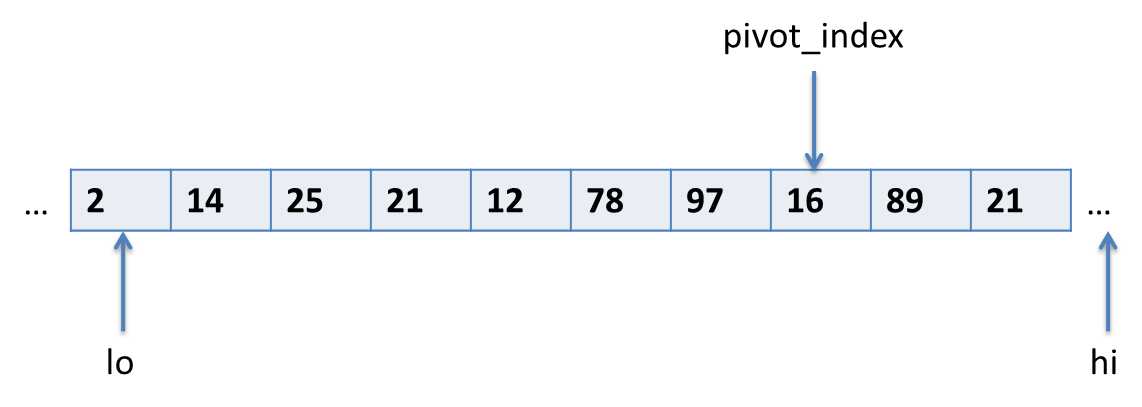
\includegraphics[width=0.85\textwidth]{img/part1.png}
\end{center}
Perhaps the first thing we notice is that we do not know where the
pivot will end up in the partitioned array!  That's because we don't
know how many elements in the segment are smaller and how many are
larger than the pivot.
In particular, the return value of partition could be different than the pivot index
that we pass in, even if the value that used to be at the pivot index in the array
before calling partition will be at the returned index when partition
is done.\footnote{To see why, imagine there are several elements equal
to the pivot value.}
One idea is to make a pass over the segment
and count the number of smaller elements, move the pivot into its
place, and then scan the remaining elements and put them into their
place.  Fortunately, this extra pass is not necessary.  We
start by moving the pivot element out of the way, by swapping
it with the leftmost element in the array segment.
\begin{center}
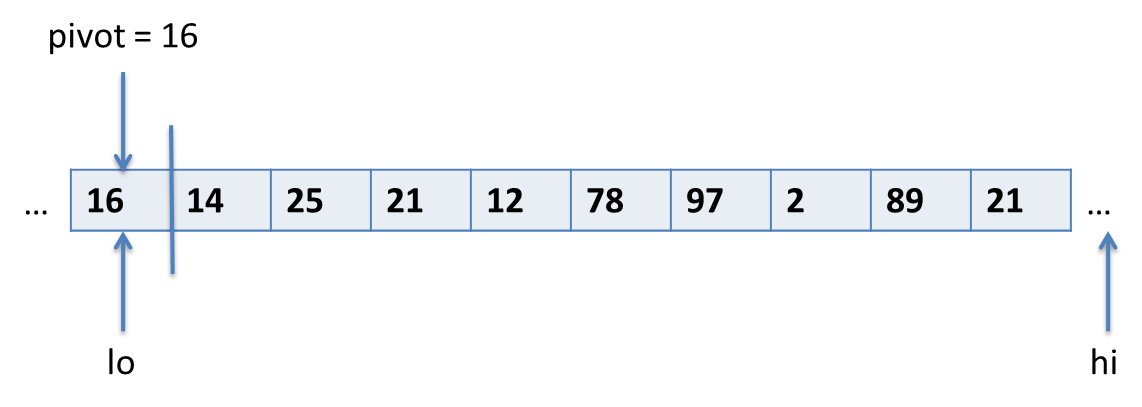
\includegraphics[width=0.85\textwidth]{img/part2.png}
\end{center}
Now the idea is to gradually work towards the middle, accumulating elements
less than the pivot on the left and elements greater than the pivot on the
right end of the segment (excluding the pivot itself).  For this purpose we
introduce two indices, $\mathit{left}$ and $\mathit{right}$.  We start them
out as $\mathit{lo+1}$ (to avoid the stashed-away pivot) and
$\mathit{hi}$.
\begin{center}
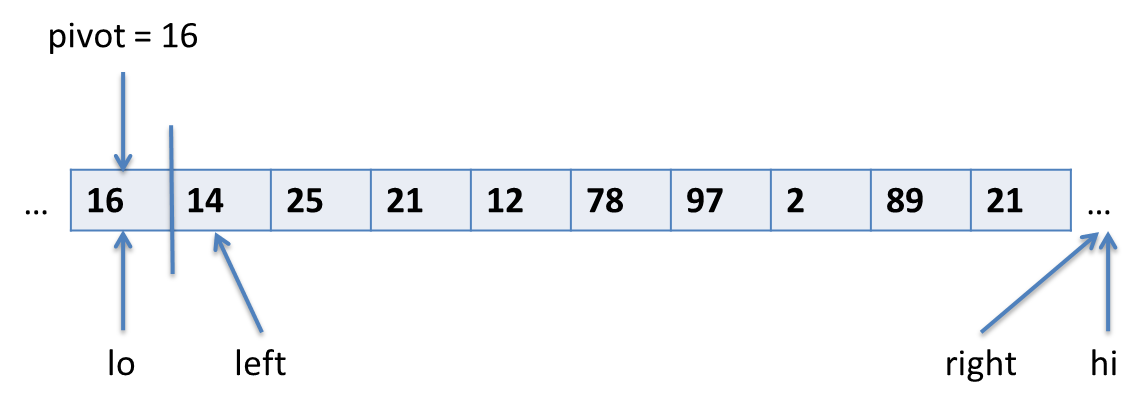
\includegraphics[width=0.85\textwidth]{img/part3.png}
\end{center}
Since $14 < \mathit{pivot}$, we can advance the $\mathit{left}$ index: this
element is in the proper place.
\begin{center}
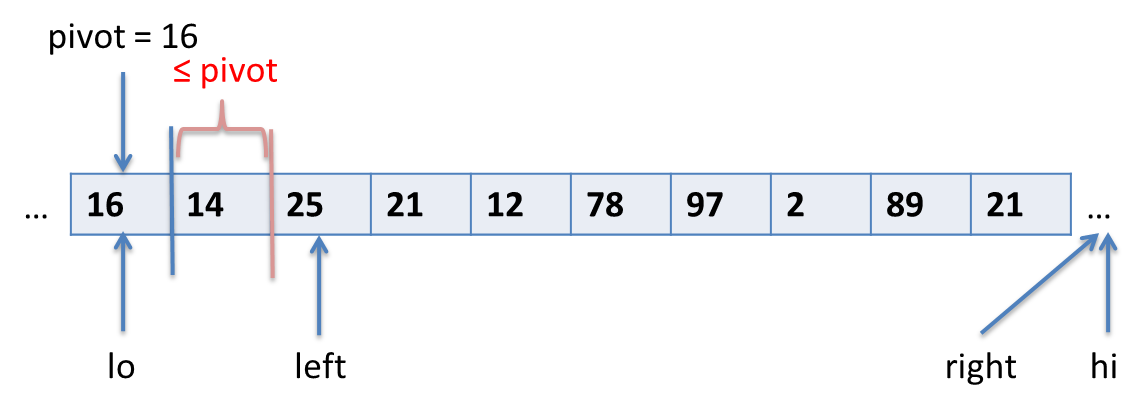
\includegraphics[width=0.85\textwidth]{img/part4.png}
\end{center}
At this point, $25 > \mathit{pivot}$, it needs to go on the right side
of the array. If we put it on the \emph{extreme} right end of the array, we
can then say that it is in its proper place.
We swap it into $A[\mathit{right-1}]$ and decrement the
$\mathit{right}$ index.
\begin{center}
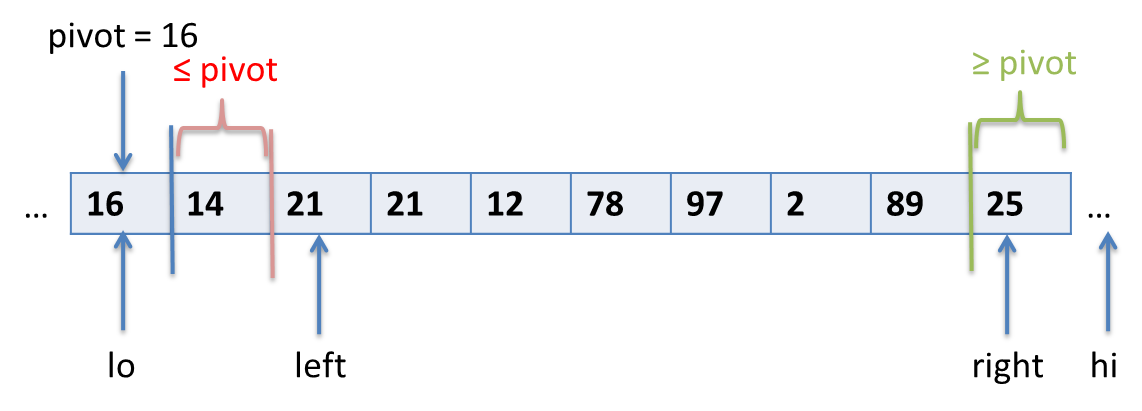
\includegraphics[width=0.85\textwidth]{img/part5.png}
\end{center}
In the next two steps, we proceed by making swaps. First, we decide
that the $21$ that is currently at $\mathit{left}$ can be properly
placed to the left of the $25$, so we swap it with the element to the
left of $25$. Then, we have $89$ at $A[\mathit{left}]$, and so we can
decide this is well-placed to the left of that $21$.
\begin{center}
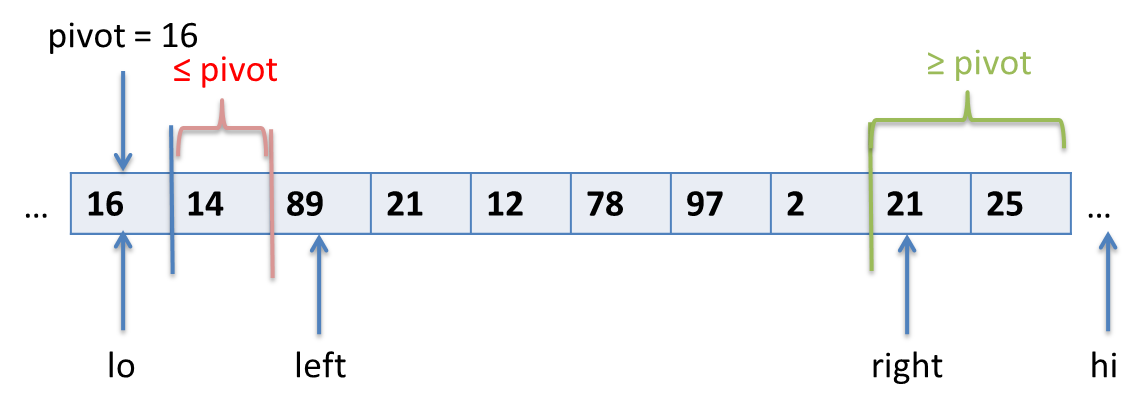
\includegraphics[width=0.85\textwidth]{img/part6a.png}
\end{center}
\begin{center}
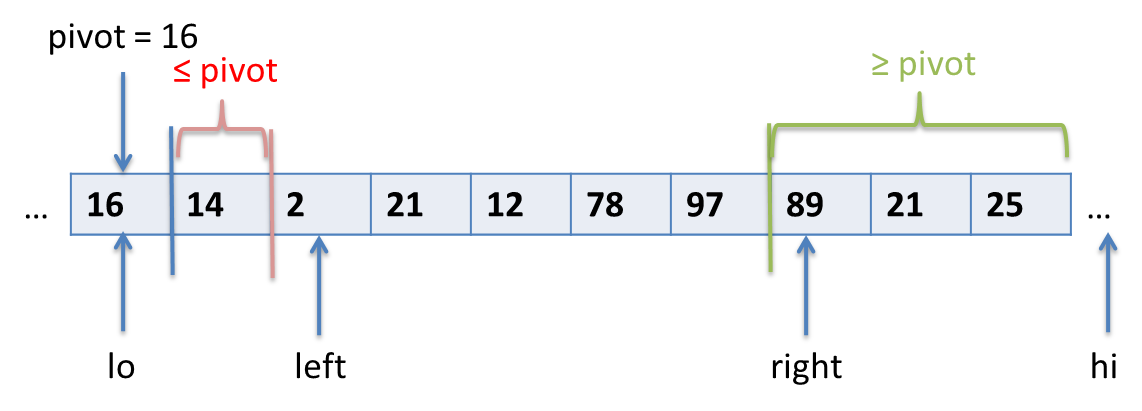
\includegraphics[width=0.85\textwidth]{img/part6b.png}
\end{center}

\noindent
Let's take one more step: $2 < \mathit{pivot}$, so we again just
decide that the $2$ is fine where it is and increment $\mathit{left}$.
\begin{center}
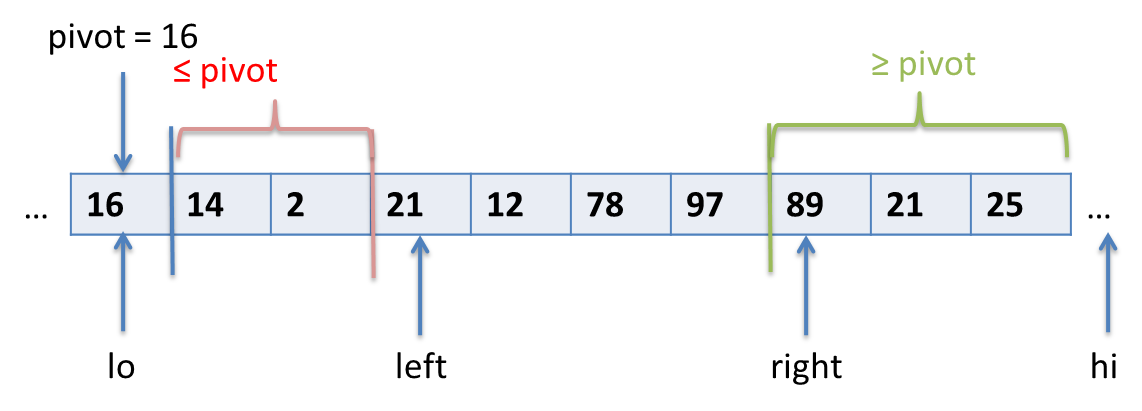
\includegraphics[width=0.85\textwidth]{img/part6c.png}
\end{center}

At this point we pause to read off the general invariants which
will allow us to synthesize the program.  We see:
\begin{enumerate}
\item[(1)] $\mathit{pivot} \geq A\lbrack\mathit{lo+1}{..}\mathit{left})$
\item[(2)] $\mathit{pivot} \leq A\lbrack\mathit{right}{..}\mathit{hi})$
\item[(3)] $A[\mathit{lo}] = \mathit{pivot}$
\end{enumerate}
We may not be completely sure about the termination condition,
but we can play the algorithm through to its end and observe:
\begin{center}
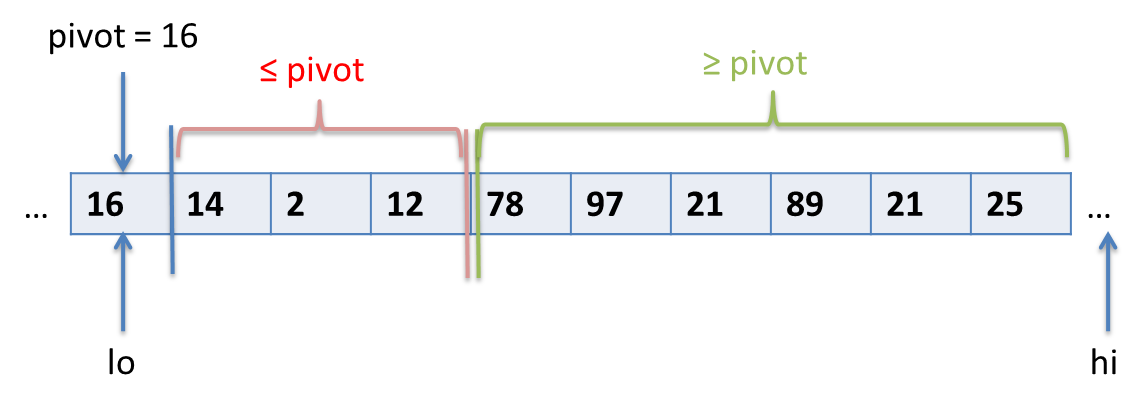
\includegraphics[width=0.85\textwidth]{img/part7.png}
\end{center}
Where do $\mathit{left}$ and $\mathit{right}$ need to be, according to our
invariants?  By invariant (1), all elements up to but excluding
$\mathit{left}$ must be less than or equal to $\mathit{pivot}$.  To guarantee
we are finished, therefore, the $\mathit{left}$ index must address the element
$78$ at $\mathit{lo}+4$.  Similarly, invariant (2) states that the pivot
must be less than or equal to all elements starting from $\mathit{right}$ up
to but excluding $\mathit{hi}$.  Therefore, $\mathit{right}$ must also
address the element $78$ at $\mathit{lo}+4$.
\begin{center}
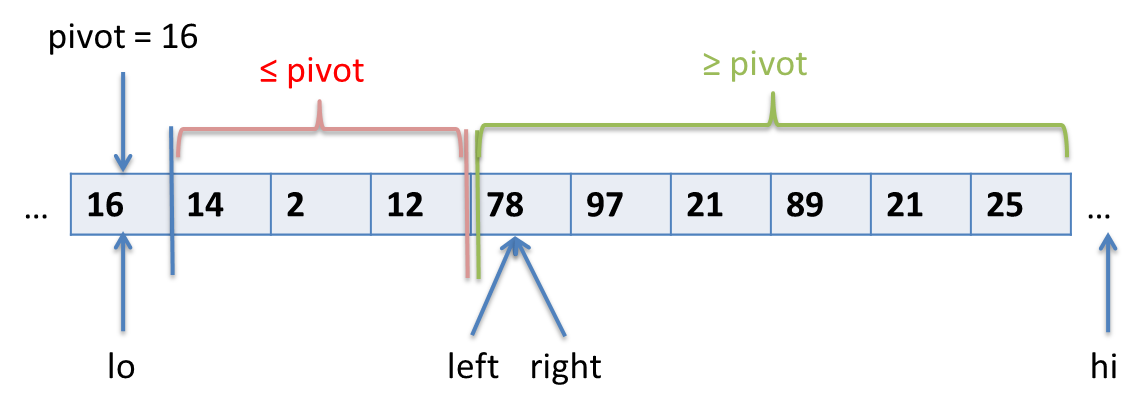
\includegraphics[width=0.85\textwidth]{img/part8.png}
\end{center}
This means after the last iteration, just before we exit the
loop, we have $\mathit{left} = \mathit{right}$, and throughout:
\begin{enumerate}
\item[(4)] $\mathit{lo}+1 \leq \mathit{left} \leq \mathit{right} \leq \mathit{hi}$
\end{enumerate}
Now comes the last step: since $\mathit{left} = \mathit{right}$,
$\mathit{pivot} \geq A[\mathit{left}-1]$ and we can swap the pivot
at $\mathit{lo}$ with the element at $\mathit{left}-1$ to
complete the partition operation.  We can also see the $\mathit{left-1}$
should be returned as the new position of the pivot element.


\section{Implementing Partitioning}
\label{sec:quicksort:impl-partitioning}
\TAGS{correctness, safety}

Now that we understand the algorithm and its correctness proof,
it remains to turn these insights into code.  We start by
swapping the pivot element to the beginning of the segment.
\begin{lstlisting}[language={[C0]C}, numbers=left]
int partition(int[] A, int lo, int pi, int hi)
//@requires 0 <= lo && lo <= pi && pi < hi && hi <= \length(A);
//@ensures lo <= \result && \result < hi;
//@ensures ge_seg(A[\result], A, lo, \result);
//@ensures le_seg(A[\result], A, \result+1, hi);
{
  // Hold the pivot element off to the left at "lo"
  int pivot = A[pi];
  swap(A, lo, pi);
  ...
}
\end{lstlisting}

\newpage
\noindent
At this point we initialize $\mathit{left}$ and $\mathit{right}$ to
$\mathit{lo+1}$ and $\mathit{hi}$, respectively.  We have to
make sure that the invariants are satisfied when we enter the loop for
the first time, so let's write these.
\begin{lstlisting}[language={[C0]C}, numbers=left, firstnumber=12]
  int left = lo+1;
  int right = hi;

  while (left < right)
    //@loop_invariant lo+1 <= left && left <= right && right <= hi;
    //@loop_invariant ge_seg(pivot, A, lo+1, left); // Not lo!
    //@loop_invariant le_seg(pivot, A, right, hi);
    {
      ...
    }
\end{lstlisting}
The crucial observation here is that $\mathit{lo} < \mathit{hi}$
by the precondition of the function.  Therefore $\mathit{left} \leq
\mathit{hi} = \mathit{right}$ when we first enter the loop.  The segments
$A\lbrack\mathit{lo+1}{..}\mathit{left})$ and $A\lbrack\mathit{right}{..}\mathit{hi})$
will both be empty, initially.

\clearpage
The code in the body of the loop just compares the element
at index $\mathit{left}$ with the pivot and either increments
$\mathit{left}$, or swaps the element to $A[\mathit{right}]$.
\begin{lstlisting}[language={[C0]C}, numbers=left, firstnumber=15]
  while (left < right)
    //@loop_invariant lo+1 <= left && left <= right && right <= hi;
    //@loop_invariant ge_seg(pivot, A, lo+1, left); // Not lo!
    //@loop_invariant le_seg(pivot, A, right, hi);
    {
      if (A[left] <= pivot) {
        left++;
      } else {
        //@assert A[left] > pivot;
        swap(A, left, right-1);
        right--;
      }
    }
\end{lstlisting}
Now we just note the observations about the final loop state with an
assertion, swap the pivot into place, and return the index $\mathit{left} -
1$.  The complete function is on the next page, for reference.

\clearpage
\begin{lstlisting}[language={[C0]C}, numbers=left]
int partition(int[] A, int lo, int pi, int hi)
//@requires 0 <= lo && lo <= pi;
//@requires pi < hi && hi <= \length(A);
//@ensures lo <= \result && \result < hi;
//@ensures ge_seg(A[\result], A, lo, \result);
//@ensures le_seg(A[\result], A, \result, hi);
{
  // Hold the pivot element off to the left at "lo"
  int pivot = A[pi];
  swap(A, lo, pi);

  int left = lo+1;
  int right = hi;

  while (left < right)
    //@loop_invariant lo+1 <= left && left <= right && right <= hi;
    //@loop_invariant ge_seg(pivot, A, lo+1, left); // Not lo!
    //@loop_invariant le_seg(pivot, A, right, hi);
    {
      if (A[left] <= pivot) {
        left++;
      } else {
        //@assert A[left] > pivot;
        swap(A, left, right-1);
        right--;
      }
    }
  //@assert left == right;

  swap(A, lo, left-1);
  return left-1;
}
\end{lstlisting}


\section{Stability}
\label{sec:quicksort:stability}
\TAGS{sorting}

Outside of introductory programming courses, much of the time, we
don't sort arrays of integers but arrays of \emph{records}, where the
data we are trying to sort (like a lecture number) is associated with
another piece of information (like a username). This is also what
happens when we tell a spreadsheet to sort by a particular column: if
we take the quicksort algorithm and try to sort the following array
by lecture number, we'll get this result:
\begin{center}
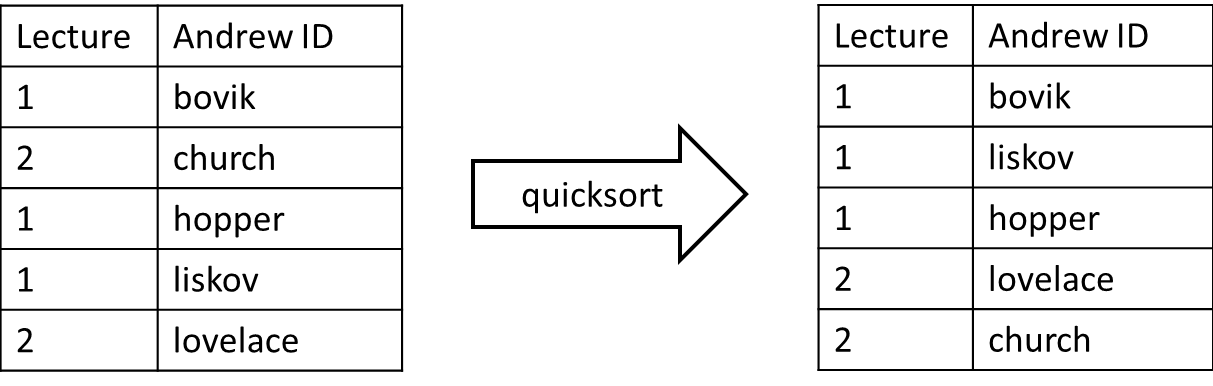
\includegraphics[width=0.85\textwidth]{img/stability-quicksort.png}
\end{center}
The resulting array \emph{is} sorted by lecture number, but whereas
\lstinline'lovelace' appeared after \lstinline'church' in the unsorted array,
they appear in the other order in the sorted array. To put it another
way, the first array is sorted by student IDs, we might expect the Andrew
IDs \emph{within} Lecture 1 and Lecture 2 to be sorted, but that's not the
case.

If a sort fulfills this expectation --- if the relative order in which distinct
elements that the sort sees as equivalent, like $(2, $\lstinline'church'$)$ and
$(2, $\lstinline'lovelace'$)$, is preserved by sorting --- then the sort is said
to be a \emph{stable sort}.
\begin{center}
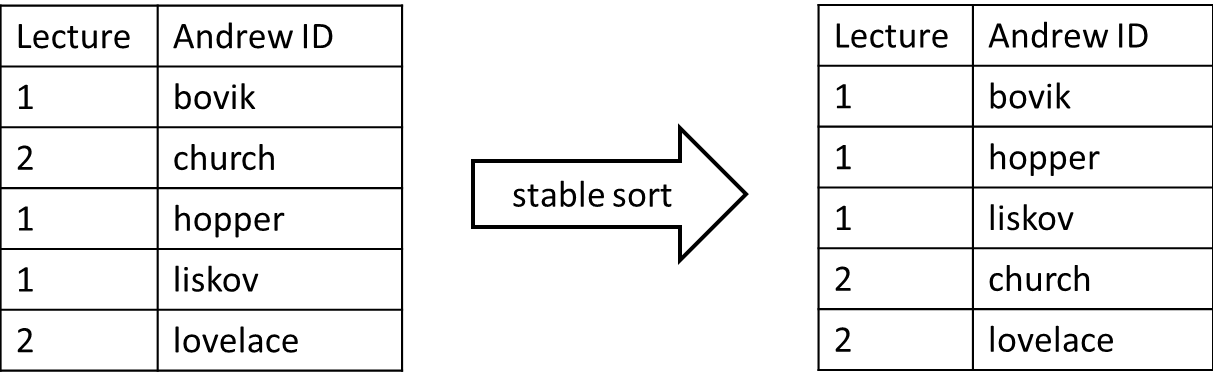
\includegraphics[width=0.85\textwidth]{img/stability.png}
\end{center}
Selection sort is in-place, slow, and not stable. Quicksort is in-place,
hopefully fast (with lucky or random pivot selection), but not
stable. We'll close out our discussion of sorting with the presentation
of a sort that's stable, fast, but not in-place.


\section{Mergesort}
\label{sec:quicksort:mergesort}
\TAGS{complexity, divide-and-conquer, sorting}

Let's think more generally about how to apply the divide-and-conquer
technique to sorting.  How do we divide? In quicksort, the partition
function is what divides the problem into two sub-problems, and it's
the first thing we do. A characteristic of mergesort is that the
\emph{divide} phase of divide-and-conquer is immediate: we only need
to calculate the midpoint.  On the other hand, it is (relatively)
complicated and expensive (linear in time and temporary space) to
combine the results of solving the two independent subproblems with
the merging operation.

The simple idea is just to divide a given array in half, sort each
half independently.  Then we are left with an array where the left
half is sorted and the right half is sorted.  We then need to
\emph{merge} the two halves into a single sorted array.  We actually
don't really ``split'' the array into two separate arrays, but we
always sort array segments $A\lbrack\mathit{lo}{..}\mathit{hi})$.  We
  stop when the array segment is of length 0 or 1, because then it
  must be sorted.

A straightforward implementation of this idea would be as follows:
\begin{lstlisting}[language={[C0]C}, numbers=left]
void sort (int[] A, int lo, int hi)
//@requires 0 <= lo && lo <= hi && hi <= \length(A);
//@ensures is_sorted(A, lo, hi);
{
  if (hi-lo <= 1) return;
  int mid = lo + (hi-lo)/2;

  sort(A, lo, mid); //@assert is_sorted(A, lo, mid);
  sort(A, mid, hi); //@assert is_sorted(A, mid, hi);
  merge(A, lo, mid, hi);
  return;
}
\end{lstlisting}
We would still have to write \lstinline'merge', of course, but compare this
to the quicksort implementation. They are very similar, but instead of
a \lstinline'partition' followed by two recursive calls, we have two
recursive calls followed by a \lstinline'merge'.  We use the specification
function \lstinline'is_sorted' from the last lecture that takes an array
segment, defined by its lower and upper bounds.

The simple and efficient way to merge two sorted array segments (so
that the result is again sorted) is to create a temporary array, scan
each of the segments from left to right, copying the smaller of the
two into the temporary array.  This is a linear time ($O(n)$)
operation, but it also requires a linear amount of temporary space.
The merge operation can be seen in the \lstinline'mergesort.c0' included as
a part of this lecture's code directory.

Let's consider the asymptotic complexity of mergesort, assuming
that the merging operation is $O(n)$.
\begin{center}
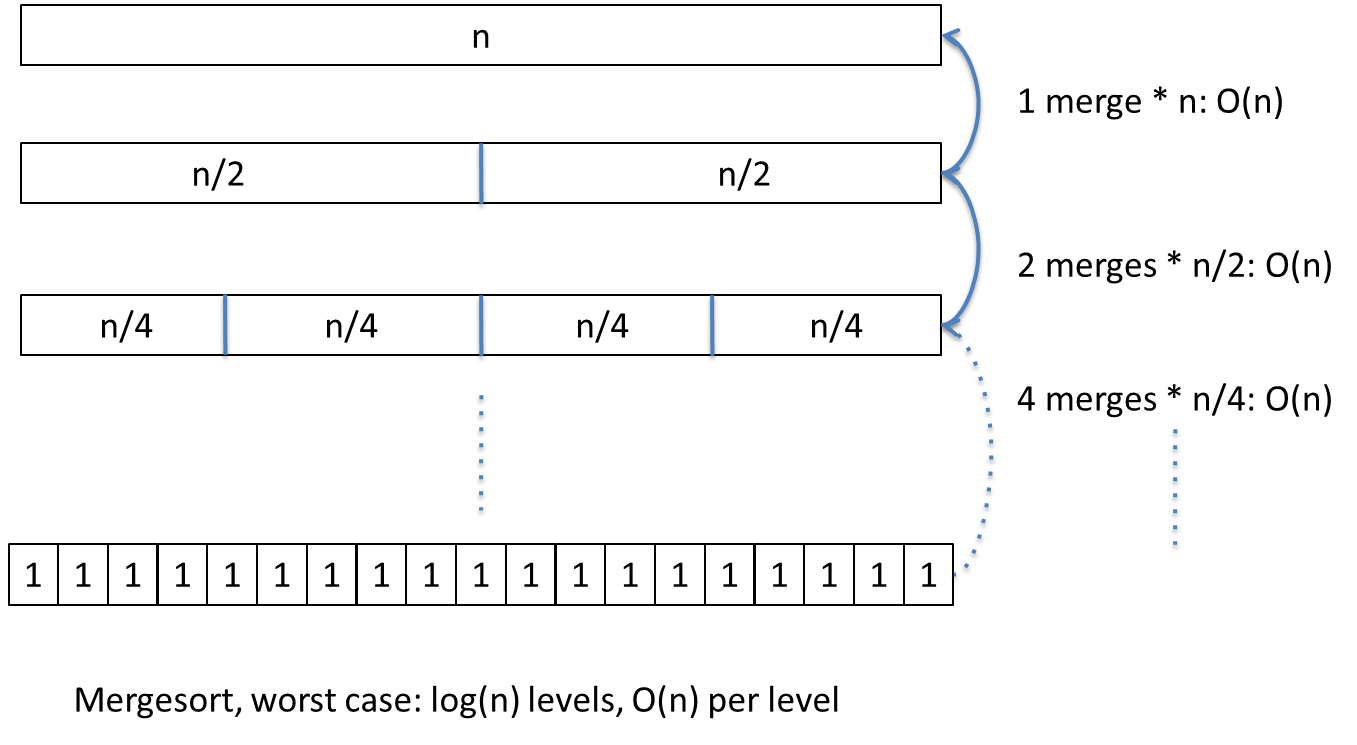
\includegraphics[width=0.99\textwidth]{img/msort1.png}
\end{center}
We see that the asymptotic running time will be $O(n \log n)$, because
there are $O(\log n)$ levels, and on each level we have to
perform $O(n)$ operations to merge.  The midpoint calculation is
deterministic, so this is a worst-case bound.


\clearpage
\section{Exercises}

\begin{exercise}
\label{exc:is-permutation}
In this exercise we explore strengthening the contracts
on in-place sorting functions.
\begin{enumerate}
\item Write a function \lstinline'is_permutation' which checks that one
  segment of an array is a permutation of another.
\item Extend the specifications of sorting and partitioning
  to include the permutation property.
\item Discuss any specific difficulties or problems that
  arise.  Assess the outcome.
\end{enumerate}
\end{exercise}

\begin{exercise}
\label{exc:qsort-post}
Prove that the precondition for \lstinline'sort' together with the
contract for \lstinline'partition' implies the post-condition.  During this
reasoning you may also assume that the contract holds for recursive
calls.
\end{exercise}

\begin{exercise}
\label{exc:partition-pess}
Our implementation of partitioning did not pick a random pivot, but
took the middle element.  Construct an array with seven elements on
which our algorithm will exhibit its worst-case behavior, that is,
on each step, one of the partitions is empty.
\end{exercise}

%% \begin{exercise}
%% \label{exc:partition-alt}
%% An alternative way to track the unscanned part of the array segment
%% during partitioning is to make the segment
%% $A[\mathit{left}{..}\mathit{right})$ exclusive on the right.

%% Rewrite the code for partition, including its invariants, for this
%% version of the indices.
%% \end{exercise}

\begin{exercise}
  An alternative way of implementing the partition function is to use extra
  memory for temporary storage. Develop such an implementation of
\begin{lstlisting}[language={[C0]C}, numbers=left]
int partition(int[] A, int lo, int pi, int hi)
//@requires 0 <= lo && lo <= pi;
//@requires pi < hi && hi <= \length(A);
//@ensures lo <= \result && \result < hi;
//@ensures ge_seg(A[\result], A, lo, \result);
//@ensures le_seg(A[\result], A, \result+1, hi);
\end{lstlisting}
\end{exercise}

\begin{exercise}
  Give an example array that shows that selection sort is not stable.
  A good way to do so is to trace the execution through the iterations
  of the loop.
\end{exercise}

% \clearpage
% \bibliographystyle{alpha}
% \bibliography{modal}
